\documentclass[conference]{IEEEtran}
\usepackage[T1]{fontenc}
\usepackage{amsmath,amssymb,booktabs,array,url}
\usepackage{algorithm,algpseudocode}
\usepackage{tikz}
\usetikzlibrary{positioning,arrows.meta,fit,calc}
\usepackage[hidelinks]{hyperref}
\hypersetup{pdftitle={FinVeritas at FinReason Cup 2026: Exact Program Execution for Verifiable Financial Reasoning and XBRL Audit Verification},
  pdfauthor={Chin-Hao Hsu}, pdfsubject={FinReason Cup 2026, Tasks 1 and 3},
  pdfkeywords={data quality rules, exact arithmetic, financial reasoning, program induction, XBRL}}

\newcommand{\DQC}[1]{DQC\,#1}
\newcommand{\QA}{\textit{Q1}}
\newcommand{\QB}{\textit{Q2}}
\newcommand{\rd}{\mathrm{rd}}
\newcommand{\Pset}{\mathcal{P}}
\hyphenation{Fin-Veritas Fin-Reason Fin-Chain Fin-Auditing}

\title{FinVeritas at FinReason Cup 2026: Exact Program Execution for Verifiable Financial Reasoning and XBRL Audit Verification}
\author{\IEEEauthorblockN{Chin-Hao Hsu}
\IEEEauthorblockA{National Tsing Hua University\\
Hsinchu, Taiwan\\
c940818s@gmail.com}}


\begin{document}
\bstctlcite{bstcontrol}
\maketitle

\begin{abstract}
Exact arithmetic cannot repair a wrong input binding. We present FinVeritas, a system for Tasks~1 and~3 of the FinReason Cup 2026 that separates binding from execution: every prediction comes from an explicit program over exact values, with inputs traceable to the question text or to facts of the filing. For verifiable financial reasoning (Task~1), programs are induced from training questions by enumerative search, replaced by computation graphs reviewed against the stated financial definitions, and complemented by question-stated formulas and by scenario programs specified from the unlabeled Test questions. For XBRL audit verification (Task~3), facts are bound by their full aspect key, and reported and calculated values come from programs for three Data Quality Committee rules, accepted under a consensus gate, with native execution of the published rules as a fallback. No language model runs at inference. FinVeritas answers 927 of the 928 Task~1 Test questions correctly and ranks joint second of 27 teams; on Task~3 it reaches 97.79\% accuracy, official rank 1 of 23 teams. Reviewed graphs change 29 Test final answers of the induced programs, and published rule programs decide 629 of the 680 Task~3 Test cases.
\end{abstract}

\begin{IEEEkeywords}
data quality rules, exact arithmetic, financial reasoning, program induction, XBRL
\end{IEEEkeywords}

\section{Introduction}
Exact arithmetic cannot correct a wrong input binding. A ratio with the wrong denominator, a growth factor applied to the wrong period, or an eXtensible Business Reporting Language (XBRL) total compared with a member fact from another context yields a wrong answer however precisely it is computed. The FinReason Cup 2026~\cite{finreason2026overview} makes this explicit. Task~1 asks for a typed final answer and named intermediate checkpoints for multi-step financial questions~\cite{finreason2026task1overview}, so a correct number reached through wrong steps is penalized. Task~3 provides an XBRL filing submitted to the U.S. Securities and Exchange Commission (SEC) and asks for two values: the value the filing reports for a target concept (\QA{}) and the value implied by the filing's own calculation or dimensional relationships (\QB{})~\cite{finreason2026task3overview}.

FinVeritas treats both tasks as one problem: bind the inputs, then execute an explicit program exactly. In Task~1 the program is a sequence of named assignments whose nodes are the required checkpoints; in Task~3 it is the logic of a published data quality rule applied to facts identified by their full aspect key. Every checkpoint and every reported value can therefore be traced to a span of the question or to a fact of the filing.

FinVeritas answers 927 of the 928 Task~1 Test questions correctly and reaches 97.79\% accuracy on Task~3. Its main contributions are:
\begin{itemize}
\item a Task~1 pipeline that induces exact-rational programs from training questions, replaces programs that fit the data but violate the stated financial identity with reviewed computation graphs, and emits checkpoints as nodes of the same program;
\item a Task~3 pipeline that binds XBRL facts by their full aspect key, accepts rule-program results only under a consensus gate, and falls back to native execution of the published Data Quality Committee (DQC) rules;
\item an evaluation that attributes every Development and Test answer to the component that produced it, measures the value of definition review on new inputs, and locates the remaining Task~3 errors by rule.
\end{itemize}

\section{Related Work}
\textbf{Financial numerical reasoning.} FinQA~\cite{chen2021finqa}, TAT-QA~\cite{zhu2021tatqa} and ConvFinQA~\cite{chen2022convfinqa} pose questions requiring arithmetic reasoning over financial reports. FinChain~\cite{xie-etal-2026-finchain} generates questions from parameterized symbolic templates over 58 topics in 12 domains and scores both final answers and step-level consistency; the Task~1 data follow this design. Program-aided approaches such as PAL~\cite{gao2023pal} and Program-of-Thoughts~\cite{chen2023pot} let a language model write code that an interpreter executes. FinVeritas also separates reasoning from computation, but obtains its programs by enumerative search against labeled examples, in the spirit of programming by example~\cite{gulwani2011flashfill}, and by reviewing them against the stated financial definitions.

\textbf{XBRL verification.} XBRL~\cite{xbrl21} encodes each reported fact with a concept, entity, period, unit and optional dimensions, and relates facts through calculation and definition linkbases. Calculations 1.1~\cite{xbrlcalc11} and the duplicate-fact guidance~\cite{xbrlduplicates} specify how summations and repeated facts are treated, and the DQC rules~\cite{dqcrules} are public consistency checks for SEC filings, executable with Arelle and its Xule processor~\cite{arelle}. FinAuditing~\cite{wang2026finauditing} builds taxonomy-structured tasks from real filings under U.S. Generally Accepted Accounting Principles (US-GAAP), including the numerical task used as the Task~3 Practice set, and reports gaps in concept retrieval and cross-document reasoning. Herculean~\cite{peng2026herculeanagenticbenchmarkfinancial} finds that agent performance depends on the financial workflow, including auditing. AuditFlow~\cite{wang2026auditflow} gives language-model agents typed tools over a taxonomy graph and the filing, and VeriFin~\cite{hall2026verifin} grounds model-generated claims in XBRL facts and checks them with an SMT solver. FinVeritas is fully symbolic at inference and reuses the published rule logic directly.

\begin{table}[t]
\caption{Data splits and their use in this work.}
\label{tab:data}
\centering\footnotesize
\setlength{\tabcolsep}{3pt}
\begin{tabular}{@{}llrp{0.46\columnwidth}@{}}
\toprule
Task & Split & Cases & Labels and use\\
\midrule
1 & Train & 2,900 & Public; program induction\\
1 & Local dev. & 290 & Public; ablation (Table~\ref{tab:ablation})\\
1 & Development & 580 & Hidden; online aggregate score\\
1 & Test & 928 & 580 seen + 348 hidden; final ranking\\
3 & Practice & 332 & Public (FinMR); parser and rule development\\
3 & Development & 680 & Hidden; online aggregate score\\
3 & Test & 680 & Hidden; final ranking\\
\bottomrule
\end{tabular}
\end{table}

\section{Tasks and Problem Formulation}
Table~\ref{tab:data} lists the data. In Task~1 each question specifies the answer type, unit and rounding, and the checkpoint slots to fill. The official scorer evaluates each case on its final answer (FAC) and its checkpoints, then averages hierarchically over templates, domain/topic/difficulty cells, difficulty levels, topics and domains. The Test set contains a seen stratum of 580 questions from training templates and a hidden stratum of 348 questions from scenario families that do not occur in training; the two strata are weighted equally in the final ranking~\cite{cupterms}.

\textbf{Task~1 formulation.} A question provides numeric literals $x=(x_0,\dots,x_n)$, an answer specification $a$ and a set $S$ of checkpoint slots. A solution is a program $P$: a sequence of named assignments $v_k=e_k(x,v_1,\dots,v_{k-1})$, a final node $v_y$ and a map $\sigma$ from slots to nodes. Its prediction is $\rho_a(v_y)$ for the final answer and $\rho_s(v_{\sigma(s)})$ for each $s\in S$, where $\rho$ renders an exact value according to a specification. Checkpoints are thus intermediate nodes of the program that produces the final answer, and the task reduces to finding $P$ and binding $x$ to its inputs.

In Task~3 each case is one query containing the schema, the presentation, calculation, definition and label linkbases, the instance document, a US-GAAP taxonomy excerpt and the question; the query does not name the rule. Each case receives exactly one label, assigned in order: structural error, extraction error (\QA{} wrong), calculation error (\QA{} correct, \QB{} wrong) or accurate. Accuracy (ACC) is the share of accurate cases, and \QB{} is compared without tolerance. The official labels are assigned by a language model (gpt-5-mini) prompted to compare the two values by their numeric meaning~\cite{task3results}. Development and Test filings come from disjoint sets of companies~\cite{task3data}. The Practice cases are labeled with the violated rule (110/120/102 cases for \DQC{0015/0117/0126}), and in all of them \QA{} and \QB{} differ.

\textbf{Task~3 formulation.} A filing is a set $F$ of numeric facts, each with an aspect key and a value $\nu(f)$, and the question names a target concept $q$ and a period $t$. Let $r\in\{0015,0117,0126\}$ be the rule the case was built around, which is not given, and $E_r(q,t)\subseteq F$ the facts of $q$ in $t$ to which $r$ applies. The answer is $\QA{}=\nu(f^*)$ for the fact $f^*\in E_r(q,t)$ that violates $r$, and $\QB{}=R_r(F,f^*)$, where $R_{0015}(F,f)=|\nu(f)|$, $R_{0117}(F,f)$ is the sum of the members of $f$ on a listed axis, and $R_{0126}(F,f)$ is the weighted sum of the calculation children of $f$. A system can therefore fail in three places: the choice of $r$, the choice of $f^*$ when several facts are eligible, and the operand set of $R_r$.

\begin{figure*}[t]
\centering
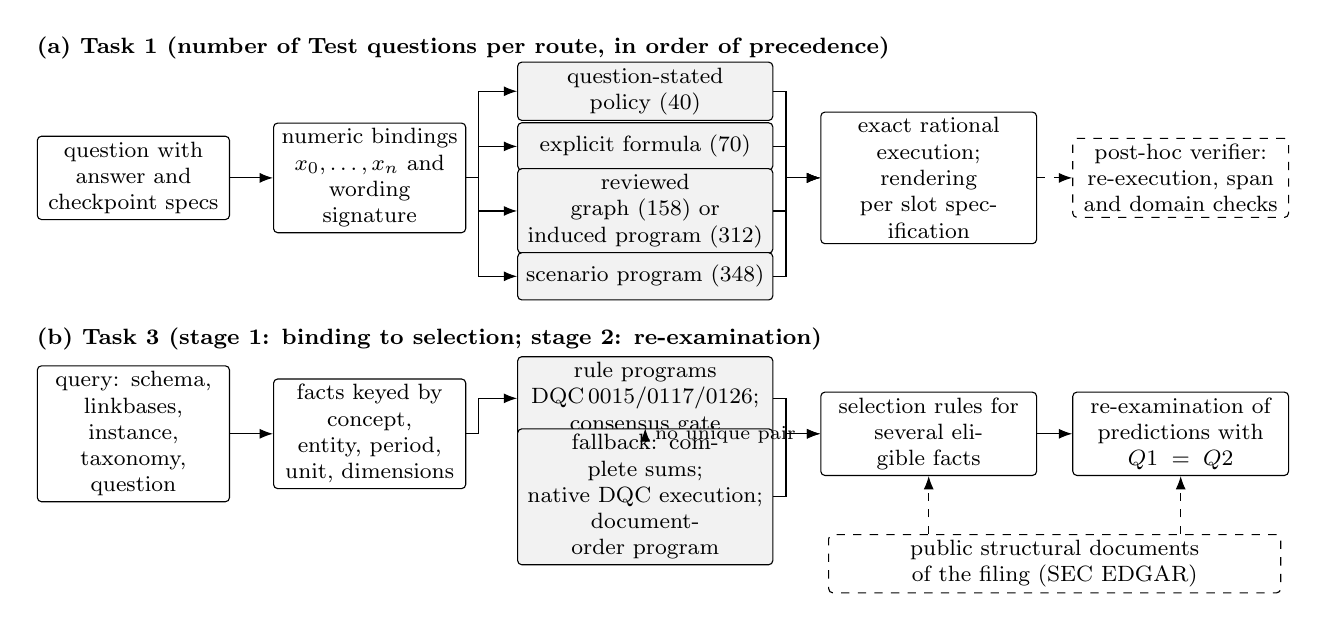
\begin{tikzpicture}[
  font=\footnotesize, >=Latex,
  box/.style={draw, rounded corners=1.5pt, align=center, inner sep=2pt, minimum height=6mm},
  route/.style={box, fill=black!5, text width=3.1cm},
  ext/.style={box, dashed},
  lab/.style={font=\footnotesize\bfseries, anchor=west}]
% ---------- (a) Task~1
\node[lab] at (-0.1,0.35) {(a) Task~1 (number of Test questions per route, in order of precedence)};
\node[box, text width=2.3cm] (q1) at (1.25,-1.3) {question with\\answer and\\checkpoint specs};
\node[box, text width=2.3cm] (b1) at (4.25,-1.3) {numeric bindings\\$x_0,\dots,x_n$ and\\wording signature};
\node[route] (p)  at (7.75,-0.2) {question-stated policy (40)};
\node[route] (e)  at (7.75,-0.9) {explicit formula (70)};
\node[route] (r)  at (7.75,-1.72) {reviewed graph (158) or\\induced program (312)};
\node[route] (h)  at (7.75,-2.55) {scenario program (348)};
\node[box, text width=2.6cm] (x1) at (11.35,-1.3) {exact rational\\execution; rendering\\per slot specification};
\node[ext, text width=2.6cm] (v1) at (14.55,-1.3) {post-hoc verifier:\\re-execution, span\\and domain checks};
\draw[->] (q1)--(b1);
\foreach \n in {p,e,r,h} {\draw[->] (b1.east) -- ++(1.6mm,0) |- (\n.west); \draw[->] (\n.east) -- ++(1.6mm,0) |- (x1.west);}
\draw[->, dashed] (x1)--(v1);
% ---------- (b) Task~3
\node[lab] at (-0.1,-3.35) {(b) Task~3 (stage 1: binding to selection; stage 2: re-examination)};
\node[box, text width=2.3cm] (q3) at (1.25,-4.55) {query: schema,\\linkbases, instance,\\taxonomy, question};
\node[box, text width=2.3cm] (b3) at (4.25,-4.55) {facts keyed by\\concept,\\entity, period,\\unit, dimensions};
\node[route] (c8)  at (7.75,-4.1) {rule programs\\\DQC{0015/0117/0126};\\consensus gate};
\node[route] (nat) at (7.75,-5.35) {fallback: complete sums;\\native DQC execution;\\document-order program};
\node[box, text width=2.6cm] (foc) at (11.35,-4.55) {selection rules for\\several eligible facts};
\node[box, text width=2.6cm] (ret) at (14.55,-4.55) {re-examination of\\predictions with\\$Q1=Q2$};
\node[ext, text width=5.6cm] (cat) at (12.95,-6.2) {public structural documents\\of the filing (SEC EDGAR)};
\draw[->] (q3)--(b3);
\draw[->] (b3.east) -- ++(1.6mm,0) |- (c8.west);
\draw[->] (c8.south) -- node[right=0pt, font=\scriptsize]{no unique pair} (nat.north);
\foreach \n in {c8,nat} {\draw[->] (\n.east) -- ++(1.6mm,0) |- (foc.west);}
\draw[->] (foc)--(ret);
\draw[->, dashed] (cat.north -| foc.south) -- (foc.south);
\draw[->, dashed] (cat.north -| ret.south) -- (ret.south);
\end{tikzpicture}
\caption{Overview of the two pipelines. Shaded boxes are program sources; all arithmetic is exact. Dashed: post-hoc verification (a) and external structural documents (b, Section~\ref{sec:source}).}
\label{fig:pipelines}
\end{figure*}

\section{Task~1: Exact Financial Programs}
Fig.~\ref{fig:pipelines}(a) shows the pipeline. A question is answered by the first applicable route, in the order question-stated policy, explicit formula, reviewed or induced program, and scenario program. Fallback routes that answer no Development or Test question are omitted here.

\subsection{Binding and wording signatures}
The question text before the answer-format block is scanned for numeric literals (integers, decimals and fractions). Each literal becomes a binding $x_i$, numbered in order of occurrence, with its exact rational value and character span. Replacing every literal by a placeholder gives the question's \emph{wording signature}. The 2,900 training questions, ten per template, have 320 signatures over 290 templates. At inference a question uses the program stored for its exact wording signature, provided the number of bindings also matches.

\subsection{Program induction}
Programs are induced per signature from the value vectors of its training questions. The search starts from the bindings and the constants $\{0,1,2,3,4,12,100,365,10000\}$ and grows a pool keyed by value vector, keeping for each vector the expression of lowest cost, then shortest length. Atoms cost 0, each unary or binary operation adds 1, closed forms cost 3--7 and reused checkpoints cost 2. The operators are negation, absolute value, $+,-,\times,\div,\min,\max$ and integer powers with $|t|\le 24$; the closed forms are $g=(1+r/100)^t$, $Ag$, $A(g-1)$, $A/g$ and $A(1-1/g)/(r/100)$ for $0\le t\le 40$. Closed-form rates must vary; amounts must vary and exceed 50 in magnitude in some training example.

Numeric checkpoints are solved first, by exact-vector lookup or the first matching binary combination, and join the pool for reuse over up to four rounds. A numeric final takes the cheapest candidate that reproduces every gold output string. If none does, one more $+,-,\times,\div$ combination of a base or checkpoint atom and a stored candidate is tried, with operand costs totaling at most 9, and the first match is accepted. Categorical finals and checkpoints seek a consistent sign-to-label map when labels vary. Algorithm~\ref{alg:induction} summarizes the numeric branch. Induction yields numeric finals for 209 signatures and categorical rules for 16; the remaining 95 (36 policy, 21 explicit-formula and 38 other signatures) are covered by later routes.

\subsection{Reviewed financial graphs}
Ten training questions do not always determine the intended relationship (Section~\ref{sec:reviewed}). For 79 templates we therefore transcribed the definition given in the question text, for example variants of the weighted average cost of capital (WACC), Lintner dividend smoothing or one-period binomial option pricing, into a small graph of named assignments, a final expression and a map from checkpoint slots to nodes. A reviewed graph replaces the induced program of its template whenever one exists.

\subsection{Question-stated computations}
Two question families state their computation in the text. Policy questions begin with a fixed preamble (``Apply only this fictional scenario-local \ldots''), define thresholds and flags, and ask for one of several categorical outcomes; the policy route recognizes 20 such policies by their checkpoint identifiers and evaluates the stated comparisons. Explicit-formula questions begin with ``Use exact arithmetic.'', assign named variables and print the formula; the explicit route recognizes the printed formula among 31 known forms and evaluates it and its checkpoint subexpressions over the named variables. Questions a route does not recognize fall through to the reviewed or induced program. On Test the policy route answers 40 of the 100 policy questions and the explicit route 70 of the 148 explicit-formula questions.

\begin{algorithm}[t]
\caption{Numeric program induction for one wording signature}
\label{alg:induction}
\small
\begin{algorithmic}[1]
\Require training questions $q_1,\dots,q_m$ of the signature with bindings $x^{(j)}$ and gold answers
\Ensure checkpoint expressions $\{e_s\}$ and a final expression $e_y$, or failure
\State $B\gets$ deduplicated binding and constant atoms; $V\gets$ their value vectors
\State expand $V$ with unary, binary and filtered closed forms from $B$, keeping the cheapest expression per vector
\For{round $=1,\dots,4$}
  \For{each unsolved numeric checkpoint $s$ with gold vector $g_s$}
    \If{$g_s\in V$ or $g_s=a\circ b$ with $a,b\in V$, $\circ\in\{+,-,\times,\div\}$}
      \State $e_s\gets$ first matching expression; add it to $B$ and $V$ with reuse cost 2
    \EndIf
  \EndFor
  \State stop if no checkpoint was solved; otherwise expand $V$ using checkpoint atoms and $B$
\EndFor
\State $e_y\gets$ cheapest $v\in V$ with $\rho_a(v_j)=\rho_a(\text{gold}_j)$ for all $j$
\State if absent, take the first matching bounded binary extension described above
\State \Return $(\{e_s\},e_y)$, or failure if $e_y$ remains absent
\end{algorithmic}
\end{algorithm}

\subsection{Scenario programs for the hidden stratum}
The 348 hidden-stratum Test questions come from 116 multi-stage scenario families of three questions each, such as stress-tested capital decisions, three-stage ratchets or comparisons of financing plans. These families do not occur in training, so induction cannot reach them. We specified one program per family from the unlabeled Test question text, using AI coding assistants and without answer feedback. A program consists of a marker phrase, the expected number of numeric literals, named intermediate assignments, a final expression and one expression per checkpoint; categorical decisions are conditional expressions. A program applies only if its first checkpoint identifier, marker phrase, checkpoint count and literal count all match the question and no other program does. Literals are bound in order of occurrence, and Boolean flags are read from fixed phrases.

\subsection{Execution, rendering and verification}
All routes evaluate expressions with whitelisting interpreters over Python \texttt{Fraction}s. The main interpreter accepts integer literals, bindings, the four arithmetic operations, $\min$, $\max$, absolute value, floor, ceiling, comparisons, integer powers up to 120 and geometric sums of up to 120 terms. Values stay exact until rendering, which applies each slot's specification: rounding half away from zero at the stated number of decimals, or an exact value. Rendered values are never reused, so rounding cannot propagate between checkpoints.

A separate verifier checks every prediction after inference: identifiers and checkpoint sets must match the question, numeric values must be finite, categorical values must lie in their allowed sets, and each binding's character span must still contain its literal. A second, independently written interpreter re-executes the reviewed and induced programs.

\textbf{FinChain use.} We used the public FinChain repository (commit \texttt{9bd2942}) only as a reference for the operator vocabulary and the closed forms of the search space. No FinChain template is matched and no FinChain code is executed at inference, so FinChain contributes to no prediction directly.

\begin{algorithm}[t]
\caption{Task~3 inference for one case}
\label{alg:task3}
\small
\begin{algorithmic}[1]
\Require query with filing $F$, target concept $q$ and period $t$
\Ensure answer pair $(\QA{},\QB{})$
\State parse $F$; bind facts by aspect key; normalize $t$
\State $\Pset\gets$ violating programs of \DQC{0015}, 0117 and 0126 for the facts of $q$ in $t$
\If{the consensus gate, Eq.~\eqref{eq:gate}, accepts $\Pset$}
  \State $y\gets$ the agreed pair
\ElsIf{one non-dimensional target has all calculation children}
  \State $y\gets$ its complete Calculations 1.1 sum
\Else
  \State $d\gets$ document-order program; $n\gets$ bound native finding
  \State $y\gets n$ if $n$ exists and is consistent with $d$, else $d$
\EndIf
\State $y\gets$ selection rules (Section~\ref{sec:selection}) applied to $y$
\If{$\QA{}=\QB{}$ in $y$}
  \State $y\gets$ re-examination of $y$ (Section~\ref{sec:reexam})
\EndIf
\State \Return $y$
\end{algorithmic}
\end{algorithm}

\subsection{Example}
A local-development question~\cite{finreason2026task1overview} asks for the disposal gain or loss of an asset costing USD 100,000, with zero residual value and a nine-year useful life, sold for USD 65,000 after nine months plus four full years of straight-line depreciation. Binding gives $x_0{=}100000$, $x_1{=}9$, $x_2{=}9$, $x_3{=}4$, $x_4{=}65000$. Induction recovers only $x_0/x_1$; the reviewed graph supplies the rest:
\begin{align*}
a &= x_0/x_1 = 100000/9,\\
d &= a\,(x_2/12 + x_3) = 475000/9,\\
c &= x_0 - d = 425000/9,\\
y &= x_4 - c = 160000/9.
\end{align*}
The three checkpoints $a$, $d$ and $c$ are emitted exactly, and only the final value is rounded, to \texttt{17777.78}. All four values match the reference.

\section{Task~3: Rule-Bound XBRL Verification}
Fig.~\ref{fig:pipelines}(b) and Algorithm~\ref{alg:task3} give the pipeline: a first stage of rule programs, fallbacks and selection rules, and a second stage that re-examines predictions with $\QA{}=\QB{}$.

\subsection{Parsing and fact binding}
Each query is split into its sections, and every XML section is parsed with entity expansion, document type definition (DTD) loading and network access disabled. Concepts are identified by their expanded name (namespace URI and local name), never by prefix spelling. A numeric fact $f$ is bound to the key
\begin{equation}
k(f)=(q_f,\,e_f,\,t_f,\,u_f,\,\delta_f),
\label{eq:key}
\end{equation}
with concept $q_f$, entity $e_f$, period $t_f$, unit $u_f$ and the set $\delta_f$ of explicit and typed dimension members. Facts with equal keys are duplicates. Following~\cite{xbrlduplicates}, duplicates with equal declared decimals must have equal values, and duplicates with different decimals are consistent if their rounding intervals intersect; a consistent group is reduced to its most precise fact, and an inconsistent group blocks the programs that would use it. Nil facts are not treated as zero. Periods are compared with the period equality of XBRL 2.1, in which an instant denotes the end of the day it names.

\subsection{Rule programs and consensus gate}
\DQC{0015} requires that concepts on its published non-negative list, outside its axis and member exclusions, are not reported negative; for an eligible negative fact, \QA{} is the reported value and \QB{} its absolute value, following the benchmark's correction convention~\cite{task3results}. \DQC{0117} compares a total with the sum of its members on the rule's listed axes, holding all other dimensions fixed and letting a reported subtotal replace its descendants. \DQC{0126} compares a statement total with the weighted sum of its direct calculation children, which must all be present and aspect-aligned. Sums are computed over exact rationals. A \DQC{0117} or 0126 program reports a violation when the reported value $v$ and the computed value $R$ differ beyond the rounding tolerance of the published rules,
\begin{equation}
|\rd_d(v)-\rd_d(R)|>m\cdot 10^{-d},
\label{eq:tolerance}
\end{equation}
where $\rd_d$ rounds half to even at $d$ decimals; for \DQC{0117}, $d$ is the smallest declared decimals of the total and its members, at most 5, and $m=2$; for \DQC{0126}, $d$ is the declared decimals of the total and $m=n+1$ for $n$ addends. Values exactly on a rounding boundary are left undecided.

Since the query does not name the rule, every program applicable to a target fact is evaluated. Let $\Pset(c)$ be the applicable programs that report a violation for case $c$. The consensus gate accepts a pair only when these programs agree:
\begin{equation}
y(c)=
\begin{cases}
(r,s) & \text{if } \{(r_p,s_p):p\in\Pset(c)\}=\{(r,s)\},\\
\bot & \text{otherwise,}
\end{cases}
\label{eq:gate}
\end{equation}
where $\bot$ passes the case to the fallbacks. The gate also requires that the target facts lie in a single entity and unit scope and that no duplicate group of the target is inconsistent. When \DQC{0117} admits several axes, each axis is a separate program, so a pair is accepted only if all admissible axes imply it.

\subsection{Fallbacks}
For $y(c)=\bot$, three fallbacks are tried in order. First, a unique non-dimensional target with all calculation children uses its complete Calculations 1.1 sum~\cite{xbrlcalc11}. Second, the original DQC US rule bodies~\cite{dqcrules} run with Arelle 2.46.1 and Xule~\cite{arelle} in a fresh offline workspace, using a reduced taxonomy and the asked period. A native finding must match the target concept, context, unit and period, and its reported value must equal the sole value of that concept in that context and unit in the supplied instance. Its \QB{} is the magnitude for \DQC{0015} or the message's sum for \DQC{0117/0126}. A native pair is used only if it is unique and its \QA{} agrees with the third fallback, when that fallback has a candidate. The third fallback takes the first eligible negative target fact in document order and its magnitude.

\subsection{Selection rules}
\label{sec:selection}
Some filings report several eligible facts for the target concept, one per legal entity, plan, debt facility or segment, and the question does not say which is meant. Seventeen selection rules, developed with Development feedback, handle such cases. Seven are triggered by a property of the filing or target, such as an ownership axis or the concept \texttt{PaymentsForRestructuring}; the others prefer, for example, the state-and-local tax scope, a postretirement plan type, the legal-entity member whose value is uniquely negative, or the revolving facility whose value changes least across periods, and some refer to extension members of a particular issuer. They change 17 Development output pairs and no Test output pair.

\subsection{Re-examination of unchanged predictions}
\label{sec:reexam}
In every labeled Practice case \QA{} and \QB{} differ, and the organizers' extraction-only baseline, which outputs $\QB{}=\QA{}$, scores 0\% on Development~\cite{task3results}. A prediction with $\QB{}=\QA{}$ therefore indicates that no violation was found, and the second stage examines such cases again. This stage was built for the Test submission, whose first-stage output contained 17 such predictions. For \DQC{0015} targets with eligible negative facts in the asked period, the most frequent eligible negative value (ties: smallest magnitude) is taken as \QA{} and its magnitude as \QB{}. Other cases are examined with progressively weaker evidence, stopping at the first step that yields a finding:
\begin{enumerate}
\item native execution with the filing's original structural documents (Section~\ref{sec:source}) and the supplied instance;
\item native execution with the supplied documents, treating disclosure roles as statement roles, since the native \DQC{0117} assertion applies to statement cubes;
\item our own \DQC{0117} program on the supplied documents, which tries definition-tree members first, then members absent from those networks, and takes the last candidate axis in the fixed DQC rule order.
\end{enumerate}
A native step is accepted when it yields a single finding bound to the target fact, or several of which the \DQC{0117} program selects one. No Development prediction has $\QB{}=\QA{}$ after the first stage, so this stage changes no Development output pair; it changes 17 Test output pairs: 6 by the \DQC{0015} rule and 8, 2 and 1 by the three steps.

\subsection{External resources}
\label{sec:source}
Besides the case query, inference reads public DQC sources and concept lists, generic taxonomies from xbrl.org, FASB and the SEC, and a fixed catalog of schema and linkbase documents from 36 SEC EDGAR filings of 25 companies. These are the structural documents of 16 Development and 20 Test filings; they are not shipped with the cases. Documents are matched by entity, target namespace and schema reference, then hash-checked. They contain no instance documents or data-quality findings, so all filing facts used to produce the answers come from the supplied instance. Withholding them changes seven Development outputs, all among the 17 changed by selection rules, and no Test output before re-examination, whose first step uses them for eight Test outputs.

\begin{table}[t]
\caption{Facts of NotesPayableCurrent in the Practice example.}
\label{tab:example}
\centering\footnotesize
\setlength{\tabcolsep}{3pt}
\begin{tabular}{@{}llr@{}}
\toprule
Instant & Dimension (axis: member) & Value\\
\midrule
2024-03-31 & none & 2,400,000\\
2024-03-31 & RelatedPartyTransactions\ldots: Shareholder & 475,050\\
2024-03-31 & RelatedPartyTransactions\ldots: OtherAffiliates & 110,500\\
2024-03-31 & DebtInstrument: CEOandCFOAdvances & 3,490\\
2023-03-31 & none & nil\\
2023-03-31 & RelatedPartyTransactions\ldots: Shareholder & 222,771\\
2023-03-31 & RelatedPartyTransactions\ldots: OtherAffiliates & nil\\
2023-03-31 & DebtInstrument: CEOandCFOAdvances & 200\\
\bottomrule
\end{tabular}
\end{table}

\subsection{Example}
A Practice case~\cite{finreason2026task3overview,wang2026finauditing} of rule \DQC{0117} asks for the reported and the calculated value of \texttt{NotesPayableCurrent} on 2024-03-31. Table~\ref{tab:example} lists the eight facts of this concept in the instance; all share entity and unit (USD). The asked instant removes the four 2023 facts, and the only remaining non-dimensional fact gives $\QA{}=2{,}400{,}000$. \DQC{0117} lists the related-party axis but not the debt-instrument axis, so the program sums the two related-party members: $475{,}050+110{,}500=585{,}550$. With $d=0$ and $m=2$, the difference far exceeds the tolerance of Eq.~\eqref{eq:tolerance}, the target belongs to a balance-sheet statement cube, and no other program reports a violation, so Eq.~\eqref{eq:gate} returns $(\QA{},\QB{})=(2{,}400{,}000,\ 585{,}550)$, which matches the reference.

\section{Evaluation}
\subsection{Setup}
Both systems run offline on a single workstation with Python 3.11. Task~1 uses only the standard library; Task~3 additionally uses lxml, Arelle 2.46.1 with Xule, and the DQC US rules at revision \texttt{15523c2} (approved v29 branch). Development and Test predictions use the same code and configuration. Local-development scores use the official scorer.

\subsection{Task~1 results}
\label{sec:t1results}
FinVeritas scores 1.000000 FAC and 1.000000 checkpoint accuracy on the 580 Development questions; the organizers' model-based baselines score 0.980556/0.987725 (Standard) and 0.984444/0.990000 (Advanced)~\cite{cupterms,task1dev}. On Test~\cite{task1results} it reaches Combined FAC 0.999167, Hidden FAC 1.000000 and Combined Checkpoint 0.997500, answers 927 of the 928 questions correctly and ranks joint second of 27 teams. The Hidden FAC of 1.000000 means that all 348 hidden-stratum questions, answered by the scenario programs, are correct, so the single wrong final answer lies in the seen stratum. All Development and Test predictions pass the post-hoc verifier, whose second interpreter recomputes 1,318 values on the 470 reviewed and induced answers of each set.

\begin{table}[t]
\caption{Task~1 route ablation on the 290 local-development questions (official scorer). Each row adds one route.}
\label{tab:ablation}
\centering\footnotesize
\setlength{\tabcolsep}{3.5pt}
\begin{tabular}{@{}lrrrr@{}}
\toprule
Configuration & Finals & Slots & FAC & Checkpoint\\
\midrule
Induced programs & 218 & 449/518 & 0.7496 & 0.9020\\
+ reviewed graphs & 270 & 501/518 & 0.9419 & 0.9754\\
+ question-stated policy & 281 & 509/518 & 0.9786 & 0.9893\\
+ explicit formula & 290 & 518/518 & 1.0000 & 1.0000\\
\bottomrule
\end{tabular}
\end{table}

\subsection{Route ablation and definition review}
\label{sec:reviewed}
Table~\ref{tab:ablation} adds routes cumulatively on the 290 local-development questions. Induced programs alone answer 218 questions, all correctly; the remaining questions fail because no complete final program was found. Reviewed graphs add 52 correct answers, the largest single gain, and the two question-stated routes complete the set.

Reviewed graphs and induced programs both produce an answer for 27 local-development, 54 Development and 54 Test questions. They agree on all local-development and Development questions but disagree on 34 Test questions from 19 templates, 29 of them in the final answer. In 12 of the 34, a parameter that was constant across the ten training questions of the template takes a new value on Test, and the induced program had absorbed it into a literal; in the other 22, the induced expression agrees with the stated formula only on the training values. For example, a cross-currency question asks for euros $\times$ (USD per EUR)/(USD per GBP). In all ten training questions the first rate is twice the second, so induction returns euros $\times\,2$; a Test question quotes 1 and 2 USD, for which the stated cross rate $1/2$ gives 197 pounds, whereas the induced program would give 788. Since only one submitted Test final answer is wrong, at least 28 of the 29 reviewed final answers that differ from the induced ones are correct.

\subsection{Task~3 results}
FinVeritas reaches 100.00\% ACC on Development~\cite{task3results}. On Test it answers 665 of the 680 cases correctly and holds official rank 1 of 23 teams~\cite{task3results}; Table~\ref{tab:t3test} gives the official scores.

\begin{table}[t]
\caption{Task~3 Test results (official judge, 680 cases~\cite{task3results}). E, C: extraction and calculation error rates; the last three columns are ACC within each rule (162/54/464 cases). All values in \%.}
\label{tab:t3test}
\centering\footnotesize
\setlength{\tabcolsep}{6pt}
\begin{tabular}{@{}rrrrrr@{}}
\toprule
ACC & E & C & 0015 & 0117 & 0126\\
\midrule
97.79 & 0.29 & 1.91 & 91.36 & 98.15 & 100.00\\
\bottomrule
\end{tabular}
\end{table}

\begin{table}[t]
\caption{Task~3 initial answer sources and subsequent changes.}
\label{tab:sources}
\centering\footnotesize
\setlength{\tabcolsep}{4pt}
\begin{tabular}{@{}lrr@{}}
\toprule
Component & Development & Test\\
\midrule
Rule programs, consensus gate & 618 & 629\\
Complete Calculations 1.1 sum & 25 & 9\\
Native DQC finding & 15 & 10\\
Document-order program & 22 & 32\\
\midrule
\quad of these, changed by selection rules & 17 & 0\\
\quad of these, changed by re-examination & 0 & 17\\
\bottomrule
\end{tabular}
\end{table}

\subsection{Answer sources and agreement with the published rules}
Table~\ref{tab:sources} counts the initial answer sources before selection and re-examination, then the cases changed by those steps. Rule programs decide 629 of the 680 Test cases on their own. Native execution also informed development: our programs follow conditions from the published Xule sources, including statement cubes, listed axes, concept names and period equality, and were checked against native results.

Table~\ref{tab:native} compares the final answers with the native finding bound to the target fact, obtained by executing the published rules on every case. Where a single native finding is bound, our answer equals it in every case except two Development cases, which the judge accepts; where several are bound, the selection step decides. The 12 Test cases without a bound finding are 4 dimensionally invalid targets, 4 filings for which the rules report nothing and 4 in which they report findings for other facts only. For unique \DQC{0117} and 0126 matches the operand sets also coincide (474 Development and 487 Test cases), so the answers agree with the published rules in the facts summed as well as in value.

\begin{table}[t]
\caption{Final Task~3 answers compared with the bound native DQC finding.}
\label{tab:native}
\centering\footnotesize
\setlength{\tabcolsep}{4pt}
\begin{tabular}{@{}lrr@{}}
\toprule
Relation to native finding & Development & Test\\
\midrule
Equal to the unique bound finding & 654 & 646\\
One of several bound findings & 20 & 22\\
Different from the bound finding & 2 & 0\\
No bound finding & 4 & 12\\
\bottomrule
\end{tabular}
\end{table}

\subsection{Error analysis}
Official per-rule aggregates place 14 of the 15 Test errors in \DQC{0015} (148/162 correct), one in \DQC{0117} and none in \DQC{0126}. Only 2 cases overall are extraction errors, so at least 12 of the 14 are labeled calculation errors, although \QB{} is the negation of \QA{} under this rule. Our output contains exactly 162 pairs in the \DQC{0015} form (listed non-negative target, $\QA{}<0$, $\QB{}=-\QA{}$), the official rule count, six of them from re-examination. This pattern is consistent with errors in the bound value or its scale rather than in the negation rule itself, matching the organizers' observation that the reported value and its scale were the hard part of this task~\cite{task3results}.

\subsection{Reproducibility}
Rerunning both systems from source reproduces every submitted Task~1 record and every Task~3 value, and two Test runs of Task~3 are byte-identical. All 1,360 \QA{} values occur as facts of the asked concept and period in the supplied instance, and an audit re-derives 787 candidate-program operand-witness sums with exact rationals (391 Development, 396 Test) without arithmetic failure. Code and reproduction instructions are available at \url{https://github.com/cs113062273-bot/IEEE-FinReason-FinVeritas}.

\section{Discussion}
\textbf{Validation scores do not expose underdetermined programs.} Reviewed and induced programs agree on every shared local-development and Development question, yet diverge on 34 Test questions. Validation therefore gave no signal of the problem; only new input values did. Most disagreements are coincidental fits rather than absorbed constants, so checking constant parameters alone would miss them. Reviewing a program against the stated definition catches both kinds.

\textbf{Published rule logic decides most cases.} Rule programs written from the published definitions decide about nine in ten cases under the consensus gate, and the final answers match a bound native finding in 668 of the 680 Test cases. On unique \DQC{0117} and 0126 matches the two also agree on the operands.

\textbf{The remaining difficulty is the choice of fact.} Fourteen of the 15 Test errors occur under the rule whose \QB{} is fixed once \QA{} is chosen, and the Development cases changed by selection rules are also choices among eligible facts. This evidence suggests that the bottleneck lies in identifying $f^*$ and its scale rather than in computing $R_r$.

\textbf{Language-model selection gave no benefit.} We tested whether a frozen language model could replace the selection rules. Qwen3-14B (4-bit quantized, no fine-tuning), run locally, chose among the remaining candidate programs while all arithmetic stayed deterministic, with each candidate list presented in forward and reversed order. On the 332 Practice cases the model changed at most seven answers, with a net gain of at most one and only in the reversed order, and a variant that changes an answer only when both orders agree changed none. Its choices were not stable under candidate order, so it is not part of the submitted system.

\textbf{Limitations.} Task~1 coverage is tied to known question families: the scenario programs were specified from the Test questions, so the 348 hidden-stratum results measure scenario transcription, not generalization to unseen families. In Task~3, selection rules use Development feedback and some are issuer-specific, re-examination is heuristic, seven Development and eight Test answers depend on structural documents not shipped with the cases, and native execution uses a reduced taxonomy restricted to the asked period.

\section{Conclusion}
FinVeritas separates input binding from exact execution and runs no language model at inference. It answers 927 of 928 Task~1 Test questions correctly (joint second of 27 teams) and reaches 97.79\% on Task~3 (official rank 1 of 23). Definition review corrects programs that validation cannot distinguish, and published rule programs decide most XBRL cases.

\section*{Acknowledgment}
The author thanks the FinReason Cup organizers. This independent work received no external funding. AI disclosure: OpenAI Codex and Anthropic Claude Code were used throughout system development and paper preparation. Claude drafted all sections from the code, results and analyses and edited the language. Claude Code and Codex were used for code implementation, including the 116 scenario programs, and debugging; Codex was also used for technical revisions of Sections I--VIII and for reference and reproducibility checks. The author is responsible for the final text, claims and results.

\bibliographystyle{IEEEtran}
\bibliography{references}
\end{document}
